\chapter{CƠ SỞ LÝ THUYẾT}
\label{chap:cosolythuyet}
Chương này trình bày nền tảng để đọc kiến trúc MyTinyMobileNetSoC ở Chương~\ref{chap:kientruc} và phân tích tối ưu hóa ở Chương~\ref{chap:toiuu}. Trọng tâm là suy luận CNN số nguyên, bộ xử lý điều phối và chi phí cung cấp dữ liệu cho phần cứng.
\section{Trí tuệ nhân tạo - Artificial Intelligence}
Trí tuệ nhân tạo – Artificial Intelligence là một lĩnh vực khoa học tập trung vào việc xây dựng các máy tính và máy móc có khả năng lập luận, học hỏi và hành động theo cách mà thông thường đòi hỏi trí tuệ con người hoặc xử lý những dữ liệu có quy mô vượt quá khả năng phân tích của con người. Quá trình học này thường bao gồm các thuật toán, là tập hợp các quy tắc hoặc hướng dẫn giúp AI phân tích và đưa ra quyết định. Trong học máy (Machine Learning), một nhánh phổ biến của AI, các thuật toán được huấn luyện trên dữ liệu đã được gán nhãn hoặc chưa được gán nhãn để đưa ra dự đoán hoặc phân loại thông tin.\\
\\
Học sâu (Deep Learning), một chuyên ngành sâu hơn, sử dụng các mạng nơ-ron nhân tạo với nhiều lớp để xử lý thông tin, mô phỏng cấu trúc và chức năng của não bộ con người. Thông qua quá trình học hỏi và thích nghi liên tục, các hệ thống AI ngày càng thành thạo trong việc thực hiện các nhiệm vụ cụ thể, từ nhận dạng hình ảnh đến dịch ngôn ngữ và hơn thế nữa. Một số mạng nơ-ron nhân tạo phổ biến gồm mạng nơ-ron hồi tiếp (Recurrent Neural Networks - RNN), mạng bộ nhớ dài/ngắn hạn (Long/Short Term Memory - LSTM) và mạng nơ-ron tích chập (Convolutional Neural Networks - CNN).
Phân loại ảnh có giám sát xây dựng ánh xạ từ ảnh sang các nhãn định nghĩa trước. Trong huấn luyện, dữ liệu có nhãn được dùng để điều chỉnh trọng số và bias nhằm giảm hàm mất mát. Trong suy luận, tham số đã học được giữ cố định; hệ thống thực hiện các phép toán của mạng để tạo điểm số và chọn nhãn. Phạm vi phần cứng của luận văn là suy luận; huấn luyện và chuẩn bị tham số diễn ra bên ngoài SoC.

Tensor là mảng nhiều chiều biểu diễn ảnh, trọng số và kết quả trung gian. Với một ảnh, tensor đặc trưng có $C$ kênh, chiều cao $H$ và chiều rộng $W$; mỗi kênh là một bản đồ đặc trưng (feature map). Kích thước logic khác với thứ tự lưu bộ nhớ. Ký hiệu $X_{c,y,x}$ chỉ kênh $c$ và vị trí $(y,x)$; bố trí CHW lưu liên tiếp các phần tử không gian của từng kênh, theo thuật ngữ ở Chương~\ref{chap:kientruc}.

CNN khai thác quan hệ lân cận của dữ liệu không gian: bộ lọc quan sát vùng cục bộ và cùng trọng số được dùng tại nhiều vị trí. Các lớp liên tiếp kết hợp đặc trưng để phân loại. Tính cục bộ và chia sẻ trọng số cũng tạo cơ hội tái sử dụng dữ liệu trên phần cứng~\cite{alzubaidi2021review}.

\section{Tích chập, stride, padding và kích hoạt}
\subsection{Tích chập nhiều kênh}
Xét đầu vào $X$ kích thước $C_{\rm in}\times H\times W$ và đầu ra $Y$ có $C_{\rm out}$ kênh. Mỗi kênh đầu ra $o$ có trọng số $W_{o,c,u,v}$ kích thước $C_{\rm in}\times K_h\times K_w$ và bias $b_o$. Với stride $s_h,s_w$ và padding trên/trái $p_t,p_l$, kết quả trước kích hoạt là
\begin{equation}
 Y_{o,y,x}=b_o+\sum_{c=0}^{C_{\rm in}-1}\sum_{u=0}^{K_h-1}\sum_{v=0}^{K_w-1}
 W_{o,c,u,v}X_{c,s_hy+u-p_t,s_wx+v-p_l}.
\end{equation}
Đây là tích chập nhiều kênh: mỗi đầu ra tích lũy trên toàn bộ kênh đầu vào và vị trí kernel. Trường hợp một kênh có $C_{\rm in}=1$. Theo quy ước CNN, kernel không bị lật chỉ số; phép tính về hình thức là tương quan chéo, thường vẫn gọi là tích chập.

Stride là khoảng dịch cửa sổ giữa hai vị trí đầu ra liên tiếp. Padding bổ sung giá trị ngoài biên, thường bằng không trong miền thực, và có thể không đối xứng. Với padding dưới/phải $p_b,p_r$, không dùng dilation, kích thước đầu ra là
\begin{equation}
\begin{split}
 H_{\rm out}&=\left\lfloor\frac{H+p_t+p_b-K_h}{s_h}\right\rfloor+1,\\
 W_{\rm out}&=\left\lfloor\frac{W+p_l+p_r-K_w}{s_w}\right\rfloor+1.
\end{split}
\end{equation}
Stride lớn hơn một thường giảm độ phân giải. Padding cùng stride quyết định cách xử lý cửa sổ biên và vị trí lấy mẫu.

Một MAC (multiply--accumulate) nhân hai toán hạng rồi cộng vào tổng. Lớp trên cần khoảng $H_{\rm out}W_{\rm out}C_{\rm out}K_hK_wC_{\rm in}$ MAC, chưa tính bias và hậu xử lý. Đây là khối lượng số học, không bao gồm tải dữ liệu hoặc điều khiển.

\subsection{Kích hoạt và clamp}
Hàm kích hoạt tạo tính phi tuyến. ReLU là $\max(0,x)$; ReLU6 là $\min(6,\max(0,x))$. Khi lượng tử hóa, các cận thực phải ánh xạ sang miền nguyên tương ứng. Clamp giới hạn giá trị vào $[q_{\min},q_{\max}]$. Clamp theo toàn miền INT8 chỉ giới hạn khả năng biểu diễn, không tự tương đương ReLU hoặc ReLU6. Cần phân biệt cận kiểu dữ liệu với cận kích hoạt của mô hình.

\section{Tích chập depthwise, pointwise và tách theo chiều sâu}
\subsection{Depthwise: xử lý không gian theo từng kênh}
Với depth multiplier bằng một, depthwise convolution (DW) dùng một bộ lọc không gian riêng cho mỗi kênh đầu vào và giữ nguyên số kênh:
\begin{equation}
 D_{c,y,x}=b^{\rm DW}_c+\sum_{u=0}^{K_h-1}\sum_{v=0}^{K_w-1}
 W^{\rm DW}_{c,u,v}X_{c,s_hy+u-p_t,s_wx+v-p_l}.
\end{equation}
Các kênh được xử lý độc lập, không trộn thông tin. Stride và padding tác động lên cửa sổ như tích chập chuẩn; stride~2 có thể giảm kích thước không gian mà giữ số kênh trong trường hợp này.

\subsection{Pointwise: tích vô hướng theo chiều kênh}
Pointwise convolution (PW) là tích chập $1\times1$. Với stride~1 và không padding, tại mỗi vị trí, vector $C_{\rm in}$ phần tử được nhân với vector trọng số của từng kênh đầu ra:
\begin{equation}
 P_{o,y,x}=b^{\rm PW}_o+\sum_{c=0}^{C_{\rm in}-1}W^{\rm PW}_{o,c}D_{c,y,x}.
\end{equation}
Tích vô hướng này tạo $C_{\rm out}$ kênh, giữ kích thước không gian. Cùng trọng số được dùng lại ở mọi vị trí, tạo cơ hội giữ trọng số cục bộ.

\subsection{Chi phí của cặp DW--PW}
Depthwise-separable convolution thực hiện DW rồi PW: lọc không gian trước, trộn kênh sau. Đây là thành phần nền tảng của MobileNets~\cite{howard2017mobilenets}. Với kernel $K\times K$, depth multiplier bằng một và cùng miền đầu ra, số MAC mỗi vị trí là $K^2C_{\rm in}+C_{\rm in}C_{\rm out}$, so với $K^2C_{\rm in}C_{\rm out}$ của tích chập chuẩn. Tỷ số là
\begin{equation}
 \frac{\mathrm{MAC}_{\rm DW+PW}}{\mathrm{MAC}_{\rm dense}}=\frac{1}{C_{\rm out}}+\frac{1}{K^2}.
\end{equation}
So sánh bỏ qua bias, kích hoạt và truyền dữ liệu. Cách tách thay đổi cấu trúc tham số, không bảo đảm thay thế mọi kernel chuẩn mà giữ nguyên hàm. TinyMobileNet trong luận văn dùng các cặp DW--PW tùy biến, không phải MobileNetV2.

\section{GAP, lớp kết nối đầy đủ và quyết định phân loại}
Pooling thu gọn miền không gian. MaxPool chọn phần tử lớn nhất trong cửa sổ cục bộ và chỉ được nêu làm ngữ cảnh chung. Mạng của luận văn dùng Global Average Pooling (GAP), lấy trung bình toàn bản đồ từng kênh:
\begin{equation}
 g_c=\frac{1}{HW}\sum_{y=0}^{H-1}\sum_{x=0}^{W-1}X_{c,y,x}.
\end{equation}
GAP chuyển tensor $C\times H\times W$ thành vector $C$ phần tử. Trong miền nguyên, phép chia và ánh xạ sang kiểu đầu ra cần quy tắc làm tròn và tái lượng tử hóa.

Lớp kết nối đầy đủ (fully connected, FC) ánh xạ vector đặc trưng sang điểm số của $J$ lớp:
\begin{equation}
 s_j=b_j+\sum_{c=0}^{C-1}W^{\rm FC}_{j,c}g_c,
 \qquad \widehat{j}=\operatorname*{arg\,max}_{0\leq j<J}s_j.
\end{equation}
Chuỗi GAP $\rightarrow$ FC $\rightarrow$ điểm số $\rightarrow$ argmax tạo quyết định phân loại. Softmax có thể chuyển logits thực thành phân bố chuẩn hóa, nhưng đường suy luận của luận văn chọn argmax trực tiếp. Điểm số nguyên trước Softmax không phải xác suất. Các điểm số so sánh trực tiếp cần có thang đo và cách biểu diễn tương thích.

\section{RISC-V}
\subsection{ISA và kiến trúc load/store}
RISC-V là kiến trúc tập lệnh (instruction set architecture, ISA), xác định hành vi phần mềm quan sát, không phải một thiết kế CPU. Các lõi cùng ISA có thể khác datapath, số chu kỳ mỗi lệnh và giao tiếp bộ nhớ. RISC-V gồm tập cơ sở và các phần mở rộng để lựa chọn chức năng theo yêu cầu~\cite{waterman2014risc}.

Trong kiến trúc load/store, phép số học làm việc trên thanh ghi; load đưa dữ liệu từ bộ nhớ vào thanh ghi, store ghi trở lại. Firmware cũng có thể truy cập thanh ghi ngoại vi bằng địa chỉ MMIO. Độ rộng thanh ghi RV32 là 32 bit, cần phân biệt với độ dài mã hóa lệnh. Lệnh cơ sở RV32I dài 32 bit; phần mở rộng C có lệnh nén 16 bit và cần phần cứng giải mã tương ứng.

\subsection{Tính năng và lợi ích RISC-V}
RISC-V là một kiến trúc tập lệnh mã nguồn mở, mang lại nhiều tính năng và lợi ích vượt trội cho các ứng dụng từ vi xử lý nhúng đến các hệ thống máy tính hiệu suất cao. Dưới đây là những tính năng nổi bật và các lợi ích mà RISC-V mang lại:
\begin{enumerate}
    \item \textit{Mở và miễn phí (Open and Free):} RISC-V là một kiến trúc mã nguồn mở và miễn phí, giúp các nhà phát triển tùy chỉnh và triển khai mà không phải lo lắng về chi phí bản quyền.
    \item \textit{Tính linh hoạt và mở rộng (Flexibility and Scalability):} RISC-V hỗ trợ thiết kế vi xử lý từ các thiết bị nhúng đến hệ thống hiệu suất cao, có thể mở rộng để tối ưu hóa cho các ứng dụng đặc thù.
    \item \textit{Hiệu suất cao và tiết kiệm năng lượng (High Performance and Energy Efficiency):}
Với kiến trúc tối giản, RISC-V mang lại hiệu suất xử lý cao và tiết kiệm năng lượng, rất phù hợp cho các thiết bị di động và nhúng.
    \item \textit{Tương thích phần mềm (Software Compatibility):}
RISC-V tương thích với nhiều ngôn ngữ lập trình và hệ điều hành như Linux, giúp dễ dàng tích hợp vào hệ thống hiện có.
    \item \textit{Chi phí thấp (Low Cost):}
Không phải trả phí bản quyền, giúp giảm chi phí sản xuất và vận hành cho các thiết bị và hệ thống RISC-V.
    \item \textit{Hỗ trợ cộng đồng và phát triển mở (Community Support and Open Development):}
Cộng đồng phát triển mạnh mẽ giúp cải tiến và đổi mới kiến trúc, thúc đẩy sự hợp tác trong ngành công nghiệp bán dẫn.
    \item \textit{Tính ổn định và dài hạn (Stability and Longevity):}
Kiến trúc cơ bản của RISC-V ổn định, đảm bảo tính dài hạn cho các ứng dụng và sản phẩm.
\end{enumerate}













\subsection{Ứng dụng và xu hướng phát triển của RISC-V }
RISC-V là một kiến trúc tập lệnh mã nguồn mở đang ngày càng được áp dụng rộng rãi trong nhiều lĩnh vực công nghệ khác nhau. Sự linh hoạt và khả năng tùy chỉnh của RISC-V đã mở ra nhiều cơ hội ứng dụng, đồng thời xu hướng phát triển của nó cũng đang diễn ra mạnh mẽ. 

\subsubsection{Ứng dụng của RISC-V}
RISC-V được sử dụng trong nhiều lĩnh vực công nghệ, đặc biệt là trong các hệ thống nhúng, trí tuệ nhân tạo (AI), điện toán đám mây và máy tính hiệu suất cao. Cụ thể:

\begin{enumerate}
    \item \textit{Ứng dụng trong IoT và thiết bị nhúng:} RISC-V được sử dụng rộng rãi trong các thiết bị IoT nhờ vào khả năng tiết kiệm năng lượng và tối ưu hóa phần cứng cho các tác vụ cụ thể. Các hệ thống IoT yêu cầu hiệu suất cao nhưng tiêu thụ năng lượng thấp, và RISC-V đáp ứng được các yêu cầu này nhờ vào sự linh hoạt trong thiết kế. Vi xử lý RISC-V có thể được tùy chỉnh cho các ứng dụng nhúng, tối ưu hóa cả về kích thước bộ nhớ và khả năng xử lý.
    \item \textit{Ứng dụng trong AI và điện toán biên:} RISC-V đang được áp dụng trong các hệ thống AI, đặc biệt là ở các ứng dụng điện toán biên. Việc sử dụng RISC-V giúp giảm chi phí và tăng tính linh hoạt trong việc triển khai các thuật toán học máy nhờ khả năng tùy chỉnh phần cứng. Các bộ xử lý RISC-V chuyên dụng cho các tác vụ AI như học sâu (deep learning) và nhận dạng hình ảnh đang giúp tối ưu hóa hiệu suất và tiết kiệm năng lượng.
    \item \textit{Ứng dụng trong máy tính hiệu suất cao (HPC):} RISC-V đang được nghiên cứu và áp dụng trong các hệ thống máy tính hiệu suất cao (HPC) và điện toán đám mây. Với khả năng mở rộng và tối ưu hóa phần cứng, RISC-V có thể đáp ứng nhu cầu xử lý các tác vụ phức tạp trong các ứng dụng HPC. Việc phát triển các bộ xử lý tùy chỉnh trên nền tảng RISC-V giúp giảm chi phí và tăng hiệu suất trong môi trường điện toán đám mây.
\end{enumerate}

\subsubsection{Xu hướng phát triển của RISC-V}
Cùng với sự phát triển mạnh mẽ trong ứng dụng, RISC-V cũng đang chứng kiến những xu hướng nổi bật trong việc phát triển và áp dụng:

\begin{enumerate}
    \item \textit{Tăng cường hệ sinh thái:} Các tổ chức và công ty đang đầu tư vào việc phát triển hệ sinh thái RISC-V, bao gồm phần mềm, công cụ phát triển và tài liệu hỗ trợ, nhằm thúc đẩy việc áp dụng kiến trúc này trong ngành công nghiệp.
    \item \textit{Đổi mới trong thiết kế vi xử lý:} Các công ty như SiFive và Renesas đang phát triển các vi xử lý dựa trên RISC-V cho nhiều ứng dụng khác nhau, từ vi điều khiển đến các hệ thống máy tính hiệu suất cao, cho thấy sự linh hoạt và khả năng mở rộng của kiến trúc này.
    \item \textit{Tập trung vào bảo mật:} Với sự gia tăng các mối đe dọa an ninh mạng, RISC-V đang được phát triển với các tính năng bảo mật tích hợp, giúp bảo vệ các hệ thống và dữ liệu quan trọng.
    \item \textit{Ứng dụng trong giáo dục và nghiên cứu:} RISC-V được sử dụng ngày càng nhiều trong các chương trình giáo dục và nghiên cứu, giúp sinh viên và nhà nghiên cứu tiếp cận với công nghệ hiện đại và phát triển các giải pháp sáng tạo.
\end{enumerate}

\noindent RISC-V không chỉ là một kiến trúc tập lệnh mã nguồn mở mà còn là nền tảng mạnh mẽ cho sự phát triển và đổi mới trong nhiều lĩnh 
vực công nghệ. Với sự gia tăng ứng dụng và xu hướng phát triển mạnh mẽ, RISC-V hứa hẹn sẽ đóng vai trò quan trọng trong tương lai c
của ngành công nghiệp vi xử lý.

\subsection{Những Thách Thức Trong Thiết Kế RISC-V}

Mặc dù thiết kế mã nguồn mở mang lại nhiều lợi ích, nhưng cũng gặp không ít thách thức. Dưới đây là các thách thức chính liên quan đến ISA RISC-V:

\begin{itemize}
    \item \textit{Giấy phép (Licensing):} Các thiết kế phần cứng mã nguồn mở dưới giấy phép OSH cho phép tái sử dụng và phân phối lại. Giấy phép CERN Open Hardware License bao gồm các dạng giấy phép khác nhau, từ mạnh mẽ đến cho phép, hỗ trợ sự phát triển và ứng dụng rộng rãi.
    
    \item \textit{Tiêu thụ Năng Lượng:} Hiệu quả năng lượng rất quan trọng đối với các bộ tăng tốc ML phần cứng trong ứng dụng edge computing. Tần số hoạt động và độ phức tạp của thiết kế ảnh hưởng đến việc tối ưu hóa tiêu thụ năng lượng, điều này là cần thiết để đạt hiệu suất tốt hơn.
    
    \item \textit{Bảo Mật:} RISC-V, với vai trò là ISA mới, cần thêm nghiên cứu về các vấn đề bảo mật như bảo vệ bộ nhớ, mã hóa và ngăn chặn tấn công kênh bên. Dù vậy, nó đã cung cấp các tính năng bảo mật cơ bản và các phần mở rộng bảo mật tùy chỉnh.
    
    \item \textit{Tính Tương Thích (Interoperability):} RISC-V chưa được chấp nhận rộng rãi trong phần mềm và hệ điều hành. Mặc dù đã có công cụ biên dịch GNU hỗ trợ, việc chuyển đổi mã nguồn và xây dựng lại hệ điều hành cho RISC-V vẫn yêu cầu nỗ lực lớn từ các nhà phát triển.
\end{itemize}





\subsection{Giới thiệu về kiến trúc tập lệnh RISC-V}
\subsection{RV32I và thao tác dữ liệu nguyên}
RV32I có 32 thanh ghi nguyên 32 bit, trong đó \texttt{x0} luôn đọc bằng không, cùng bộ đếm chương trình. Các nhóm lệnh cần cho firmware gồm cộng/trừ, logic, dịch bit, so sánh, nhánh, nhảy và load/store~\cite{waterman2014risc}. Khi đọc INT8 có dấu vào thanh ghi 32 bit, mở rộng dấu giữ nguyên giá trị; mở rộng bằng không sẽ làm sai số âm. Dịch phải số học giữ bit dấu, còn dịch phải logic chèn bit không, nên có ý nghĩa khác nhau với requantization.

\paragraph{RV32M Multiply Extensi}

RV32M cung cấp các lệnh toán học để hỗ trợ các phép toán số nguyên phức tạp. Phần mở rộng này được thiết kế nhằm cải thiện hiệu suất cho các ứng dụng cần thực hiện nhiều phép tính số học như xử lý tín hiệu số và mật mã học.
\\
\textit{Các loại lệnh trong RV32M:}

\begin{itemize}
    \item \textit{Phép nhân (MUL):} Thực hiện phép nhân số nguyên giữa hai toán hạng, kết quả được lưu trong thanh ghi đích.
    \item \textit{Phép nhân giữ phần cao (MULH, MULHSU, MULHU):} Cung cấp kết quả phần cao từ các phép nhân:
    \begin{itemize}
        \item \textit{MULH:} Nhân hai số nguyên có dấu.
        \item \textit{MULHSU:} Nhân số nguyên có dấu với số nguyên không dấu.
        \item \textit{MULHU:} Nhân hai số nguyên không dấu.
    \end{itemize}
    \item \textit{Phép chia (DIV, DIVU):} Thực hiện phép chia số nguyên:
    \begin{itemize}
        \item \textit{DIV:} Chia hai số nguyên có dấu.
        \item \textit{DIVU:} Chia hai số nguyên không dấu.
    \end{itemize}
    \item \textit{Phép lấy dư (REM, REMU):} Lấy phần dư từ phép chia:
    \begin{itemize}
        \item \textit{REM:} Phần dư từ phép chia hai số nguyên có dấu.
        \item \textit{REMU:} Phần dư từ phép chia hai số nguyên không dấu.
    \end{itemize}
\end{itemize}



\paragraph{RV32A Atomic Extension}

RV32A  cung cấp các lệnh nguyên tử để hỗ trợ đồng bộ hóa giữa các tiến trình trong môi trường đa luồng. Các lệnh này đảm bảo rằng các thao tác đọc, sửa đổi và ghi vào bộ nhớ được thực hiện một cách an toàn, không bị gián đoạn, giúp duy trì tính nhất quán của dữ liệu. RV32A cung cấp hai loại lệnh nguyên tử chính:

\begin{itemize}
    \item \textit{Atomic Memory Operation (AMO):} Các lệnh này thực hiện thao tác nguyên tử trên dữ liệu trong bộ nhớ, bảo vệ dữ liệu khỏi những thay đổi không mong muốn trong suốt quá trình thực hiện.
    \item \textit{Load Reserved (LR) và Store Conditional (SC):} 
    \begin{itemize}
        \item \textit{LR}: Lệnh này đọc một \textit{word} từ bộ nhớ và đánh dấu địa chỉ bộ nhớ để theo dõi.
        \item \textit{SC}: Lệnh này lưu trữ một \textit{word} tại địa chỉ thanh ghi, nhưng chỉ thực hiện nếu địa chỉ bộ nhớ đã được đánh dấu bởi lệnh \textit{LR}, giúp đồng bộ hóa hiệu quả giữa các tiến trình.
    \end{itemize}
\end{itemize}

\begin{figure}[!h]
    \centering
    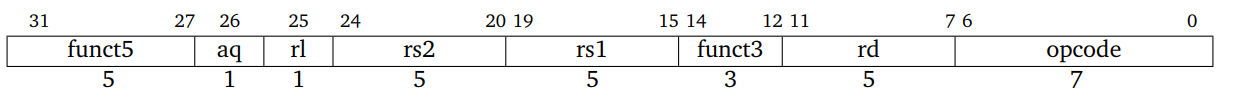
\includegraphics[width=6in]{Images/Risc-V/RV32A.png}
    \vspace{10pt} % Thay đổi giá trị 10pt theo nhu cầu
    \caption{RV32A Instruction Format}
\end{figure}

% Trong RV32A, các lệnh Atomic Memory Operations (AMO) và Load Reserved (LR) / Store Conditional \
% (SC) bao gồm:

% \begin{itemize}
%     \item \textbf{lr.w} - Load Reserved: Đọc từ bộ nhớ và đánh dấu địa chỉ.
%     \item \textbf{sc.w} - Store Conditional: Lưu dữ liệu vào bộ nhớ nếu đã được đánh dấu.
%     \item Các lệnh AMO: \textbf{amoswap.w}, \textbf{amoadd.w}, \textbf{amoand.w}, \textbf{amoor.w}, \textbf{amoxor.w}, \textbf{amomax.w}, \textbf{amomaxu.w}, \textbf{amomin.w}, \textbf{amominu.w}.
% \end{itemize}

% Những lệnh này giúp thực hiện các thao tác nguyên tử trên bộ nhớ, đảm bảo đồng bộ hóa và tính nhất quán trong môi trường đa luồng. Các lệnh nguyên tử trong RV32A đóng vai trò quan trọng trong việc phát triển các ứng dụng đa luồng và hệ thống nhúng, giúp tăng cường hiệu suất và bảo vệ dữ liệu một cách an toàn, hiệu quả.


\paragraph{RV32F / D Floating-Point Extensions }

RV32F / D cung cấp các lệnh hỗ trợ tính toán số thực tuân theo tiêu chuẩn IEEE 754, nhằm đáp ứng nhu cầu tính toán chính xác trong các ứng dụng khoa học và kỹ thuật. Các lệnh này cho phép xử lý hiệu quả dữ liệu số thực dấu phẩy động, bao gồm cả định dạng \textit{single-precision} (32-bit) và \textit{double-precision} (64-bit). RV32F / D cung cấp hai nhóm lệnh chính:

\begin{itemize}
    \item \textit{Phép toán số thực cơ bản:}  
    Các lệnh này thực hiện các phép tính cơ bản trên số thực, bao gồm cộng, trừ, nhân, chia, căn bậc hai và các phép so sánh, giúp xử lý hiệu quả các tác vụ tính toán phức tạp.

    \item \textit{Chuyển đổi định dạng:}  
    \begin{itemize}
        \item \textit{Từ số nguyên sang số thực:} Hỗ trợ chuyển đổi dữ liệu giữa số nguyên và số thực (32-bit hoặc 64-bit).  
        \item \textit{Giữa single và double precision:} Hỗ trợ chuyển đổi định dạng giữa hai loại số thực, phù hợp với yêu cầu ứng dụng.
    \end{itemize}
\end{itemize}
\\

\textit{Cơ chế đặc biệt:}  
\begin{itemize}
    \item \textit{Thanh ghi số thực:} Cung cấp 32 thanh ghi số thực (\texttt{f0} đến \texttt{f31}), kích thước 32-bit (RV32F) hoặc 64-bit (RV32D).
    \item \textit{Kiểm soát trạng thái ngoại lệ:} Các cờ trạng thái để phát hiện và xử lý các tình huống như tràn, chia cho 0 hoặc số không hợp lệ.
\end{itemize}
\\
\begin{figure}[!h]
    \centering
    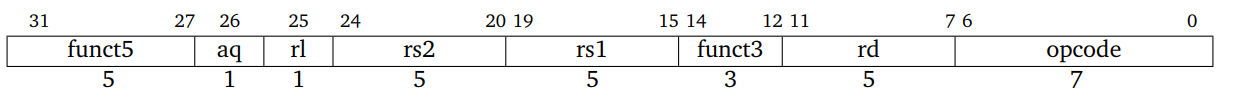
\includegraphics[width=6in]{Images/Risc-V/RV32A.png}
    \vspace{10pt} % Thay đổi giá trị 10pt theo nhu cầu
    \caption{RV32F / D Instruction Format}
\end{figure}
RV32F / D được sử dụng rộng rãi trong các ứng dụng yêu cầu tính toán số thực chính xác, như trí tuệ nhân tạo, xử lý hình ảnh, và mô phỏng khoa học, giúp nâng cao hiệu suất và tính linh hoạt của hệ thống.



\paragraph{RV32C Compressed Extension}
RV32C cung cấp các lệnh nén nhằm giảm kích thước mã lệnh và cải thiện hiệu quả sử dụng bộ nhớ trong các hệ thống nhúng hoặc ứng dụng yêu cầu bộ nhớ hạn chế. Phần mở rộng này hỗ trợ một tập hợp con các lệnh RISC-V, được mã hóa bằng 16-bit thay vì 32-bit, giúp giảm kích thước mã lệnh một cách đáng kể mà vẫn đảm bảo hiệu suất. 
\\
\\
\textit{Các tính năng chính:}
\begin{itemize}
    \item \textit{Giảm kích thước mã lệnh:}  
    RV32C sử dụng các lệnh nén 16-bit, giúp tiết kiệm bộ nhớ chương trình, đặc biệt hữu ích trong các ứng dụng nhúng và IoT.

    \item \textit{Khả năng tương thích:}  
    Các lệnh nén được thiết kế để tương thích với các lệnh 32-bit, cho phép thực thi trên cùng một kiến trúc mà không cần thay đổi phần cứng.

    \item \textit{Tối ưu hóa hiệu suất:}  
    Việc giảm kích thước mã lệnh giúp cải thiện khả năng sử dụng bộ nhớ đệm và giảm băng thông bộ nhớ, từ đó tăng hiệu suất tổng thể của hệ thống.
\end{itemize}
\textit{Phân loại các lệnh nén:}
\begin{itemize}
    \item \textit{Nén tải và lưu trữ:}  
    Cung cấp các lệnh nén để thực hiện các thao tác tải (\texttt{C.LW}, \texttt{C.LD}) và lưu trữ (\texttt{C.SW}, \texttt{C.SD}) dữ liệu.

    \item \textit{Nén các phép toán số học:}  
    Các lệnh như \texttt{C.ADD}, \texttt{C.SUB} hỗ trợ thực hiện các phép toán số học cơ bản.

    \item \textit{Nén điều kiện nhánh:}  
    Cung cấp các lệnh nén để xử lý nhánh như \texttt{C.BEQZ}, \texttt{C.BNEZ}, giúp giảm kích thước mã điều kiện
\end{itemize}
\begin{figure}[!h]
    \centering
    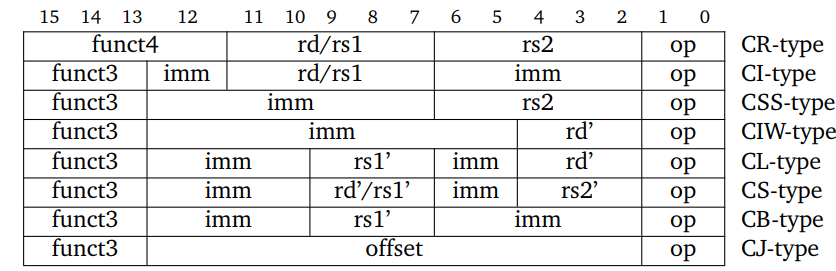
\includegraphics[width=6in]{Images/Risc-V/RV32C.png}
    \vspace{10pt} % Thay đổi giá trị 10pt theo nhu cầu
    \caption{RV32C Instruction Format}
\end{figure}
RV32C là một lựa chọn tối ưu cho các hệ thống yêu cầu mật độ mã cao, chẳng hạn như các thiết bị IoT, hệ thống nhúng và các ứng dụng yêu cầu tiết kiệm năng lượng.


\section{MMIO và phân chia phần cứng--phần mềm}
\subsection{Truy cập thanh ghi và đồng bộ hoàn tất}
I/O ánh xạ bộ nhớ (memory-mapped I/O, MMIO) đặt các thanh ghi ngoại vi trong không gian địa chỉ CPU. Lệnh load/store đến vùng này đọc hoặc ghi ngoại vi thay vì RAM. Thanh ghi có thể chứa cấu hình, toán hạng, kết quả và trạng thái; một lần ghi điều khiển có thể khởi động phép tính. CPU chỉ được dùng kết quả khi giao thức xác nhận dữ liệu hợp lệ.

Hoàn tất giao dịch bus và hoàn tất phép tính là hai sự kiện khác nhau. Ngoại vi có thể công bố cờ done/valid để phần mềm kiểm tra, hoặc trì hoãn đáp ứng lần đọc kết quả. Với giao tiếp native của PicoRV32, yêu cầu được giữ hợp lệ đến khi có ready; trong thời gian chờ, CPU chưa hoàn tất truy cập đó~\cite{YosysHQ2024}. Cơ chế này có thể gây stall mà không cần vòng polling. Ý nghĩa và vòng đời cờ trạng thái phải tuân theo giao diện từng ngoại vi.

\subsection{Chi phí offload và vai trò CPU}
Một lần gọi bộ tăng tốc gồm chuẩn bị chỉ số, nạp toán hạng, phát lệnh, chờ, đọc kết quả và hậu xử lý. Độ trễ toàn chuỗi có thể lớn hơn nhiều độ trễ datapath. Nếu mỗi phép tính nhỏ cần nhiều giao dịch, giảm số phép nhân chưa chắc giảm tương ứng chu kỳ suy luận.

Phân chia HW/SW giữ CPU phụ trách thứ tự lớp, địa chỉ tensor và xử lý đầu ra, còn phần cứng đảm nhận kernel lặp lại. Cách này linh hoạt khi đổi lịch thực thi, nhưng CPU có thể trở thành nút thắt cung cấp dữ liệu. Trong MyTinyMobileNetSoC, toán hạng đi từ RAM qua CPU tới thanh ghi bộ tăng tốc; các bộ tăng tốc không có DMA. Tái sử dụng dữ liệu cục bộ vì thế là cơ sở quan trọng cho tối ưu hóa.

\section{Tăng tốc trên FPGA, tái sử dụng dữ liệu và lập lịch}
\subsection{Tài nguyên và ràng buộc thời gian}
LUT (look-up table) hiện thực hàm logic tổ hợp; register, thường là flip-flop, giữ trạng thái qua cạnh clock. BRAM là khối bộ nhớ chuyên dụng. DSP là khối số học chuyên dụng hỗ trợ các phép như nhân và nhân--cộng. Mảng hoặc phép nhân trong RTL không tự bảo đảm được ánh xạ vào BRAM hoặc DSP; kết luận phải dựa trên báo cáo tổng hợp và hiện thực.

Chu kỳ clock $T_{\rm clk}$ là khoảng cách giữa hai cạnh hoạt động liên tiếp. Ràng buộc timing xác định thời gian cho các đường truyền, kể cả quan hệ clock và I/O. Kiểm tra setup yêu cầu dữ liệu tới thanh ghi đích đủ sớm trước cạnh lấy mẫu; slack là thời gian yêu cầu trừ thời gian đến. WNS (worst negative slack) trong báo cáo setup biểu thị slack xấu nhất theo quy ước báo cáo của công cụ: giá trị âm cho biết vi phạm; giá trị không âm cho biết các đường được phân tích đạt kiểm tra đó. Hold là kiểm tra riêng về việc giữ dữ liệu ổn định sau cạnh lấy mẫu.

Post-route tính cả ảnh hưởng định tuyến, khác với mô phỏng chức năng. Kết luận timing chỉ có giá trị trong phạm vi clock, đường truyền và điều kiện đã ràng buộc, phân tích. Một điểm đạt timing không xác nhận mọi đường đều được ràng buộc đầy đủ hoặc thiết kế đã hoạt động trên bo mạch.

\subsection{Giảm điều khiển và lưu lượng dữ liệu}
Loop unrolling mở rộng thân vòng lặp để giảm cập nhật biến đếm và nhánh; trong phần cứng, nó còn có thể tạo phép tính song song với chi phí tài nguyên cao hơn. Data packing ghép nhiều phần tử nhỏ vào một word để tăng dữ liệu hữu ích trên mỗi lần tải hoặc giao dịch. Giải gói phải giữ đúng thứ tự phần tử và mở rộng dấu.

Batching gom nhiều kết quả vào một lần gọi để chia sẻ việc nạp dữ liệu, trigger và chờ. Tiling chia miền tính toán thành vùng nhỏ phù hợp nơi lưu cục bộ. Các cửa sổ tích chập lân cận dùng chung phần tử đầu vào; nhiều kênh đầu ra có thể dùng chung một patch. Đổi thứ tự vòng lặp giúp giữ dữ liệu lâu hơn thay vì nạp lại.

Lưu trọng số cục bộ hoặc cache cho phép dùng cùng trọng số qua nhiều vị trí không gian. Cache chuyên biệt có thể được firmware nạp chủ động, không nhất thiết có cơ chế thay thế tự động như cache CPU. Lợi ích phụ thuộc dung lượng, miền tái sử dụng và chi phí chọn dữ liệu. Tăng lưu trữ hoặc song song hóa có thể tăng mux, độ dài đường tổ hợp và áp lực timing.

Mục tiêu chung là giảm truy cập RAM/MMIO và điều khiển trên mỗi kết quả hữu ích. Khi một thành phần được tăng tốc, tỷ trọng các thành phần còn lại tăng lên: đó là sự dịch chuyển nút thắt (bottleneck migration). Cần đo lại sau mỗi thay đổi; số MAC, số giao dịch và số chu kỳ là những đại lượng khác nhau.

\section{Thuật ngữ hiệu năng và kiểm chứng}
\subsection{Chu kỳ, độ trễ và đối chứng}
Cycle count là số chu kỳ giữa hai mốc đo xác định. Latency là thời gian từ đầu vào hoặc yêu cầu tới đầu ra tương ứng. Với cùng miền clock và chu kỳ đã biết, thời gian khoảng đo là $t=N_{\rm cycle}T_{\rm clk}$. Cần nêu phép đo có bao gồm UART, truyền dữ liệu, chuẩn bị đầu vào hay khởi tạo hay không. Chu kỳ mô phỏng kết hợp với ràng buộc clock chưa phải độ trễ đo trên bo mạch.

Speedup được định nghĩa bởi $S=t_{\rm baseline}/t_{\rm candidate}$. Có thể dùng tỷ số chu kỳ khi hai phiên bản có cùng chu kỳ clock. Baseline phải xác định phiên bản phần mềm, phần cứng, dữ liệu và phạm vi đo. So với CPU-only và so với hệ thống đã tăng tốc là hai phép so sánh khác nhau. Khi clock thay đổi, giảm chu kỳ chưa chắc giảm thời gian thực.

Một kết quả post-route timing-clean chỉ xác nhận đạt các kiểm tra trong flow và ràng buộc đã dùng. Điểm đạt có tần số cao nhất trong các lần thử chưa phải tần số tối đa thực sự (Fmax); kết luận Fmax cần khảo sát và điều kiện đánh giá tương ứng.

\subsection{Độ chính xác và mức độ tương đương}
Classification accuracy là tỷ lệ dự đoán đúng nhãn chuẩn trên tập đánh giá. Prediction agreement là tỷ lệ hai cách thực thi cho cùng nhãn dự đoán trên cùng đầu vào, dù nhãn đó có thể sai. Hai vector điểm số khác nhau vẫn có thể cùng argmax; đồng thuận dự đoán không xác nhận số học giống từng bit.

Tested equivalence chỉ biểu thị tương đương trên các ca đã thử, theo tiêu chí cụ thể như tensor, điểm số hoặc dự đoán. Bit-exact arithmetic equivalence đòi hỏi kết quả số nguyên trùng từng bit trong miền đầu vào xét, kể cả trường hợp làm tròn và tràn. RTL equivalence là quan hệ tương đương giữa các mô tả phần cứng theo ánh xạ trạng thái, giao diện và giả thiết môi trường xác định; chứng minh hình thức có phạm vi khác việc chạy một số testbench.

Độ chính xác phân loại, đồng thuận dự đoán và tương đương số học từng bit là ba tiêu chí riêng. Báo cáo kiểm chứng cần nêu đối tượng so sánh, dữ liệu, mức quan sát và giới hạn bằng chứng. Mô phỏng đúng chức năng cũng không thay thế kiểm tra timing hoặc thử nghiệm vật lý.
